% TO-DO:
% * (Curry-Howard) currently cannot allow implications as propositions
% * explain model-based stuff
% * dependent type theory
% * fuzzy
% * 

\documentclass[orivec]{llncs}
\usepackage{graphicx}
\usepackage{amsmath}	% for "cases"
% \usepackage{amsfonts}	% for frakur fonts
\usepackage{amssymb}    % for \rightsquigarrow, \blacksquare
\usepackage{stmaryrd}	% \llbracket
%\usepackage{mathtools}
% \usepackage{mathrsfs}	% for curly "E" error symbol
\usepackage{float}
\usepackage{comment}
% \usepackage[most]{tcolorbox}	% for wrapping example in color box
% \usepackage{wrapfig}		% wrap figure beside text, used in example
\usepackage{tikz-cd}		% commutative diagrams
% \usepackage{tikz}
% \usepackage{amssymb}		% for \multimap, \updownarrow, \bigstar
\usepackage{sectsty}		% change section color
\usepackage{hyperref}	% refs, links become clickable
\usepackage[normalem]{ulem} 	% underline unbroken with \uline

\usepackage[backend=biber,style=numeric]{biblatex}
\bibliography{../AGI-book}
% \bibliographystyle{plain} % or number or aaai ...

% \usepackage{listings}		% for algorithm
% \lstset{
%	basicstyle=\footnotesize\ttfamily,
%	mathescape
% }

% *************** Delete when not using Chinese or colors **********************
\usepackage{xeCJK}
\setCJKmainfont[BoldFont=SimHei,ItalicFont=KaiTi]{SimSun}
\usepackage{color}
%\newcommand{\emp}[1]{\textbf{\textcolor{blue}{#1}}}
\newcommand{\emp}[1]{\textbf{#1}}

\renewcommand{\labelitemi}{\textbullet}
\renewcommand{\labelitemii}{\textendash}

%\sectionfont{\color{blue}} 
%\subsectionfont{\color{blue}} 
%\subsubsectionfont{\color{blue}} 
%\definecolor{green}{rgb}{0,0.7,0}
%\definecolor{grey}{rgb}{0.95,0.95,0.95}

\usepackage{geometry}		% change paper size
\geometry{
  a4paper,         % or letterpaper
  textwidth=18cm,  % llncs has 12.2cm
  textheight=27cm, % llncs has 19.3cm
  heightrounded,   % integer number of lines
  hratio=1:1,      % horizontally centered
  vratio=2:3,      % not vertically centered
}
% \usepackage[fontsize=13pt]{scrextend}

\newcommand{\tikzmark}[1]{\tikz[overlay,remember picture] \node (#1) {};}

\newcommand{\vect}[1]{\boldsymbol{#1}}
\newcommand*\sigmoid{\vcenter{\hbox{
\includegraphics{sigmoid.png}}}}
\newcommand*\KB{\vcenter{\hbox{
\includegraphics{KB-symbol.png}}}}
\newcommand*\bbTheta{\vcenter{\hbox{\includegraphics[scale=0.75]{../bbTheta.png}}}}
% \newcommand*\rectifier{\vcenter{\hbox{\includegraphics{rectifier.png}}}}
\newcommand{\dashh}{\textemdash~}
\newcommand{\english}[1]{\rmfamily \textit{``#1''}\rmfamily}
\makeatletter
\newcommand{\logical}[1]{\mathbb{\@car#1\@nil}\mathrm{\expandafter\@cdr#1\@nil}}
\makeatother

\newcommand{\witness}{\scalebox{0.6}{$\blacksquare$}}

\newcommand{\underdash}[1]{%
	\tikz[baseline=(toUnderline.base)]{
		\node[inner sep=1pt,outer sep=10pt] (toUnderline) {#1};
		\draw[dashed] ([yshift=-0pt]toUnderline.south west) -- ([yshift=-0pt]toUnderline.south east);
	}%
}%

% ***** Boxed variables inside math equations
% \newcommand*{\boxedcolor}{black}
\makeatletter
% \renewcommand{\boxed}[1]{\textcolor{\boxedcolor}{%
% \fbox{\normalcolor\m@th$\displaystyle#1$}}}
% \setlength{\fboxsep}{1pt}
\renewcommand{\boxed}[1]{\fbox{\m@th$\displaystyle\scalebox{0.9}{#1}$} \,}
\makeatother

\overfullrule=0mm

\newsavebox{\MyName}
\savebox{\MyName}{
\includegraphics[scale=0.6]{YKY.png}}

\title{AGI via Combining Logic with Deep Learning}
\author{
%\usebox{\MyName} 
甄景贤 (King-Yin Yan) 
% \\ \footnotesize{General.Intelligence@Gmail.com}
}
\institute{General.Intelligence@Gmail.com}

\begin{document}

\maketitle

\setlength{\parindent}{0em}
\setlength{\parskip}{2.8ex plus0.8ex minus0.8ex}
% \setlength{\parskip}{2.8ex}

\begin{abstract}
An integration of deep learning and symbolic logic is proposed, based on the Curry-Howard isomorphism and categorical logic.  The propositional structure of logic is seen as a symmetry, namely the permutation invariance of propositions;  This can be implemented using so-called symmetric neural networks.  Under our interpretation, it turns out that Google's BERT, which many currently state-of-the-art language models are derived from, can be regarded as a special form of logic.  This BERT-like structure can be incorporated under a reinforcement-learning framework to form a minimal AGI architecture.  We also mention some insights gleaned from category and topos theory that point to future directions and may be helpful to other researchers, including mathematicians interested in AGI.
\end{abstract}

\begin{keywords}
deep learning, symbolic logic, logic-based AI, neural-symbolic integration, Curry-Howard isomorphism, category theory, topos theory, fuzzy logic
\end{keywords}

\setcounter{section}{-1}
\section{Introduction}
\label{sec:0}

Results in the present paper does not make use of category theory in any significant way (nor the Curry-Howard isomorphism, for that matter).  Its main accomplishment is to express AGI in the categorical language.  To the lay person, concepts of category theory (such as pullbacks, adjunctions, fibration, toposes, sheaves, ...) may be difficult to grasp, but they are the mathematician's ``daily bread''.  We hope that describing AGI in categorical terms will entice more mathematicians to work on this important topic.

Secondly, an abstract formulation allows us to see clearly what is meant by ``the mathematical structure of logic'', without which logic is just a collection of strange rules and axioms, leaving us with a feeling that something may be ``amiss'' in our theory.

\subsection{The Curry-Howard Isomorphism}

As the risk of sounding too elementary, we would go over some basic background knowledge, that may help those readers unfamiliar with this area of mathematics.

The Curry-Howard isomorphism expresses a connection between logic \textbf{syntax} and its underlying \textbf{proof} mechanism.  Consider the mathematical declaration of a \textbf{function} $f$ with its domain and co-domain:
\begin{equation}
f: A \rightarrow B .
\end{equation}
This notation comes from type theory, where $A$ and $B$ are \textbf{types} (which we can think of as sets or general spaces) and the function $f$ is an \textbf{element} in the function space $A \rightarrow B$, which is also a type.

What the Curry-Howard isomorphism says is that we can regard $A \rightarrow B$ as a \textbf{logic} formula $A \Rightarrow B$ (an implication), and the function $f$ as a \textbf{proof} process that maps a proof of $A$ to a proof of $B$.

The following may give a clearer picture:
\begin{equation}
\label{eqn:Curry-Howard}
\begin{aligned}
\boxed{\mbox{logic}} \quad \quad \underdash{$A \Longrightarrow B$} & \\
\boxed{\mbox{program}} \quad \quad \witness \; \stackrel{f}{\longmapsto} \; \witness \hspace*{10pt} & .
\end{aligned}
\end{equation}
What we see here is a logic formula ``on the surface'', with an underlying proof mechanism which is a \textbf{function}, or $\lambda$-calculus term.  Here the $\witness$'s represent proof objects or \textbf{witnesses}.  The logic propositions $A$ and $B$ coincide with the \textbf{domains} (or \textbf{types}) specified by type theory.  Hence the great educator Philip Wadler calls it ``propositions as types''. \footnote{See his introductory video: https://www.youtube.com/watch?v=IOiZatlZtGU .} 
Other textbooks on the Curry-Howard isomorphism include: \cite{Sorensen2006} \cite{Simmons2000} \cite{Thompson1991}.

The gist of our theory is that Deep Learning provides us with neural networks (ie. non-linear functions) that serve as the proof mechanism of logic via the Curry-Howard isomorphism.  With this interpretation, we can impose the mathematical structure of logic (eg. symmetries) onto neural networks.  Such constraints serve as \textbf{inductive bias} that can accelerate learning, according to the celebrated ``No Free Lunch'' theory \cite{Wolpert1997} \cite{Alpaydin2020} \cite{Shalev-Shwartz2014}.

In particular, logic propositions in a conjunction (such as $A \wedge B$) are commutative, ie. invariant under permutations, which is a ``symmetry'' of logic.  This symmetry essentially decomposes a logic ``state'' into a set of propositions, and seems to be a fundamental feature of most logics known to humans.  Imposing this symmetry on neural networks gives rise to symmetric neural networks, which can be easily implemented thanks to a separate result by other researchers.  This is discussed in \S\ref{sec:commutative-structure}.

We have not been clear about what the \textbf{proof witnesses} are.  In our current implementation, types are regions in vector space and witnesses are just points inside the regions.  When some propositions imply another proposition, there is a function mapping witnesses in some regions to a new witness in another region.  Thus, such spatial regions are nearly tautologous with proof witnesses (ie. points versus the regions containing them).  In other words, the ``big'' vector space is divided into many small regions representing various propositions.

We should point out that the Curry-Howard isomorphism has not played a significant role in our current AGI theory.  The representation of \textbf{conditional} statements (eg. $A \Rightarrow B$) requires \textbf{function types} which are hard to represent as vectors.  So the only function type in our system is the ``main'' neural network simulating the $\vdash$ operator.  In the language of classical logic-based AI, this is similar to having  ``Horn form'' logic rules in the knowledge base, acting on \textit{atomic} propositions only.

As an aside, the Curry-Howard isomorphism also establishes connections to diverse disciplines.  Whenever there is a space of elements and some operations over them, there is a chance that it has an underlying ``logic'' to it (see eg. Baez and Stay's ``Rosetta Stone'' paper: \cite{Baez2010}, also \cite{Heunen2019}).  For example, in quantum mechanics, that of Hilbert space and Hermitian operators.  Another example: in String Theory, strings and cobordisms between them (The following is the famous ``pair of pants'' cobordism, representing a process in time that merges two strings into one (time is read upwards)):
\begin{equation}
\vcenter{\hbox{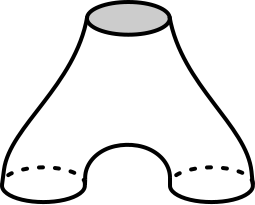
\includegraphics[scale=0.15]{pair-of-pants.png}}}
\end{equation}
Seeing logical types as topological spaces is also the origin of Voevodsky's \textbf{Homotopy Type Theory} (HoTT) \cite{Voevodsky2013}, where the \textbf{identity} of two inhabitants in a type is seen as a homotopy \textbf{path}.  HoTT may be relevant to AGI if we want the convenience of having multiple identical proofs of the same propositions -- this may help simplify the topology of types (ie. spatial regions representing propositions).

\section{Prior Research}

\subsection{Neuro-Symbolic Integration}

There has been a long history of attempts to integrate symbolic logic with neural processing, with pioneers such as Ron Sun, Dov Gabbay, Barbara Hammer, among others.  We consider two \textbf{model-based} approaches below.

From a categorical perspective, model theory is a \textbf{functor} mapping logic syntax to algebraic objects and operations between them (hence the name ``functorial semantics''):

\begin{equation}
\boxed{\mbox{syntax}} \quad
\tikzmark{a1} a \tikzmark{c1} \; {\color{red}\cdot} \; \tikzmark{b1} b \longmapsto \llbracket \tikzmark{a2} a \rrbracket \tikzmark{c2} \; {\color{red}\cdot} \; \llbracket \tikzmark{b2} b \rrbracket
\quad \boxed{\mbox{algebraic objects, eg. group elements}}
\begin{tikzpicture}[overlay, remember picture, distance=1.1cm]
\draw[->, out=40, in=135, transform canvas={shift={(4pt,10pt)}}] (a1.center) to (a2.center);
\draw[->, out=40, in=135, transform canvas={shift={(4pt,10pt)}}] (b1.center) to (b2.center);
\draw[->, out=-30, in=-140, transform canvas={shift={(6pt,-2pt)}}, red] (c1.center) to (c2.center);
\end{tikzpicture}
\end{equation}

Model theory is interesting when the target structure has additional properties not specified by the logic syntax.  For example, the predicate \texttt{male(x)} may be modelled by:
\begin{equation}
\label{table:modelling-schemes}
\begin{tabular}{|c|c|c|} \hline
algebraic geometry & \texttt{male}(x) $ \Leftrightarrow f(x) \ge 0$ & $f$ is a polynomial \\
linear algebra & \texttt{male}(x) $ \Leftrightarrow M x \ge 0$ & $M$ is a matrix \\
topology & \texttt{male}(x) $ \Leftrightarrow x \in S $ & $S$ is an open set \\
\hline
\end{tabular}
\end{equation}
Model-based methods may appear impractical for AGI because the number of grounded atomic propositions is too large (potentially infinite, if we include also propositions that are imagined).  However, if all possible atoms are embedded in a mathematical space through mapping schemes such as the above (\ref{table:modelling-schemes}), it may be approximately feasible.

In the \textbf{type-theoretic} or ``syntactic'' approach  (including the one in this paper), propositions (= types) are regions in some vector space.  Currently our simple scheme is to map predicates like $P(a,b)$ into the Cartesian product $\logical{Pred} \times \logical{Obj} \times \logical{Obj}$ where $\logical{Pred}$ is the space of all possible predicates and $\logical{Obj}$ the space of all possible objects \footnote{Here objects mean logical or first-order objects, not categorical objects} (but this is not the only option; see \S\ref{sec:dependent-types}).  \textbf{Inference} is performed by a neural network simulating the single-step consequence operator $\vdash$, while \textbf{learning} is through changing of network weights.  This is relatively simple and straightforward.

Whereas, in the \textbf{model-theoretic} approach one places objects in a high-dimensional space such that their positions satisfy the constraints imposed by various predicates (eg. polynomials, matrices, open sets, ...)  Now \textbf{inference} occurs as the system pays \textit{attention} to some points in an $\logical{Object}$ space, which points are covered by some predicates, thus forming propositions, leading to awareness of new propositions, ... and so on.  It is interesting that, under this scheme, it seems as if all truths are known \textit{a priori}, and the system just needs to pay attention to them.  \textbf{Learning} changes the geometric shapes of predicates and thus forms new truths to be discovered by the system.

\begin{enumerate}
	\item In Pascal Hitzler and Anthony Seda's \textbf{Core Method} \cite{Hitzler2011}, an \textbf{interpretation} $\mathcal{I}$ is a function that assigns truth values to the set of all possible ground atoms in a logic language $\mathcal{L}$.  One can see $\mathcal{I}$ as an enumeration of ground atoms that are true, and thus it provides a model to interpret any logic formula in $\mathcal{L}$.  Moreover $\mathcal{I}$ is a function from the space $X$ of atoms to $\mathbf{2} = \{ \top, \bot \}$ and can be given a topology $\mathbf{2}^X$ which is $X$ copies of the discrete topology of $\mathbf{2}$.  Such a topology makes $\mathcal{I}$ homeomorphic to the \textbf{Cantor set} in $[0,1]$. To a logic program $P$ is associated a \textbf{semantic operator} $\mathcal{T}_P : \mathcal{I} \rightarrow \mathcal{I}$, performing a single step of forward \textbf{inference}.  Finally, the space of interpretations $\mathcal{I}$ is embedded into $\mathbb{R}$ using a ``level mapping'' (The level of an atom increases by each inference step;  All the atoms of an interpretation $\mathcal{I}$ are translated into a fractional number in base $b$).  This allows $\mathcal{T}_P$ to be approximated by a neural network $f: \mathcal{I} \rightarrow \mathbb{R}$.  \\
	The goal of their research is to find the fixed-point semantics of logic programs, but with suitable modifications, the same mathematical structure may be used to build an inference engine or AGI.  In such case, the logic program would function as the \textbf{knowledge base} while interpretations would play the role of \textbf{working memory} (though the memory could only be a subset of an interpretation, due to physical limitation).

	\item \textbf{$\partial$-ILP} \cite{Evans2017} is focused on the learning problem, but its set-up seems similar to the first example.  A \textbf{valuation} is a vector $[0,1]^n$ mapping every ground atom to a real number $\in [0,1]$.  Each clause is attached with a Boolean flag to indicate whether it is included in the results or not.  From each clause $c$ one can generate a function $\mathcal{F}_c$ on valuations that implements a single step of forward \textbf{inference}.  To enable differentiability, the Boolean flag is relaxed to be a continuous value and gradient descent is used to \textbf{learn} which clauses should be included.
\end{enumerate}

We would also like to mention Geoffrey Hinton's recent \textbf{GLOM theory} \cite{Hinton2021}, which addresses the problem of representing a hierarchy of visual structures.  OpenCog has also been applied to neural-symbolic integration \cite{Goertzel2009} \cite{Potapov2019}.  These further support that representing and learning \textbf{relational} (logical) knowledge is a topic of central importance, and that there is a convergence of ``mainstream'' AI with AGI.

\subsection{Cognitive Architectures and Reinforcement Learning}

\textbf{Reinforcement Learning (RL).}  In the 1980's, Richard Sutton \cite{Sutton1984} introduced reinforcement learning as an AI paradigm, drawing inspiration from Control Theory and Dynamic Programming.  In retrospect, RL already has sufficient generality to be considered an AGI theory, or at least as a top-level framework for describing AGI architectures.

\textbf{Relation to AIXI.}  AIXI is an abstract AGI model introduced by Marcus Hutter in 2000 \cite{Hutter2005}.  AIXI's environmental setting is the external ``world'' as observed by some sensors.  The agent's internal model is a universal Turing machine (UTM), and the optimal action is chosen by maximizing potential rewards over all programs of the UTM.  In our (minimal) model, the UTM is \textit{constrained} to be a neural network, where the NN's \textbf{state} is analogous to the UTM's \textbf{tape}, and the optimal weights (program) are found via Bellman optimality.

\textbf{Relation to Quantum mechanics and Path Integrals.}  At the core of RL is the Bellman equation, which governs the update of the utility function to reach its optimal value.  This equation (in discrete time) is equivalent to the Hamilton-Jacobi equation in differential form.  Nowadays they are unified as the Hamilton-Jacobi-Bellman equation, under the name ``optimal control theory'' \cite{Liberzon2012}.  In turn, the Hamilton-Jacobi equation is closely related to the Schr\"{o}dinger equation in quantum mechanics:
\begin{equation}
\boxed{\mbox{Bellman eqn.}} \leftrightsquigarrow \boxed{\mbox{Hamilton-Jacobi eqn.}} \leftrightsquigarrow \boxed{\mbox{Schr\"{o}dinger eqn.}}
\end{equation}
but the second link is merely ``heuristic'';  it is the well-studied ``quantization'' process whose meaning remains mysterious to this day.  Nevertheless, the \textbf{path integral} method introduced by Richard Feynmann can be applied to RL algorithms, eg. \cite{Kappen2007}.

The Hamilton-Jacobi equation gives the RL setting a ``symplectic'' structure \cite{Mann2018};  Such problems are best solved by so-called symplectic integrators (proposed by 冯康 (Feng Kang) in the 1980s \cite{Feng2010}, see also \cite{Leimkuhler2004}).  Surprisingly, in the RL / AI literature, which has witnessed tremendous growth in recent years, there is scarcely any mention of the Hamilton-Jacobi structure, while the most efficient heuristics (such as policy gradient, experience replay, Actor-Critic, etc.) seem to exploit other structural characteristics of ``the world''.

\section{The Mathematical Structure of Logic}

Currently, the most mathematically advanced and satisfactory description of logic seems to base on category theory, known as categorial logic and topos theory.  This direction was pioneered by William Lawvere in the 1950-60's.  The body of work in this field is quite vast, but we shall briefly mention some points that are relevant to AGI.  A more detailed tutorial on categorical logic, with a focus on AGI, is in preparation \cite{Yan2021}.

\subsection{Predicates and Dependent Type Theory}
\label{sec:dependent-types}

The Curry-Howard isomorphism identifies \textit{propositional} intuitionistic logic with type theory.  As such, the arrow $\rightarrow$ in type theory is ``used up'' (it corresponds to the implication arrow $\Rightarrow$ in intuitionistic logic).  However, predicates are also a kind of functions (arrows), so how could we accomodate predicates in type theory such that Curry-Howard continues to hold?  This is the idea behind Martin L\"{o}f's \textbf{dependent type theory}.

In dependent type theory, a predicate $P(\cdot)$ is a \textbf{type constructor} (\cite{Sorensen2006} \S8.7) taking an element $a$ of one type to create a new type $P(a)$.  For example, each element $a \in \{ \text{John, Socrates, Kermit} \}$ creates a new type Human$(a)$, and thus $\mathrm{Human}$ is a \textbf{family} of types or a \textbf{dependent type}:
\begin{equation}
\label{fig:dependent-type}
\vcenter{\hbox{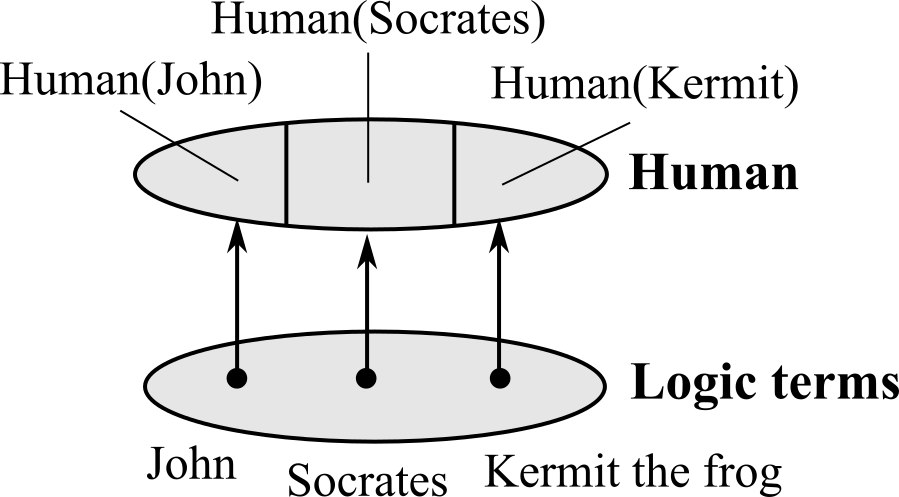
\includegraphics[scale=0.45]{dependent-type.png}}}
\end{equation}
Mathematically, a dependent type is a product of types \textbf{indexed} by another type, denoted $\Pi_A B$, which is really a form of \textbf{exponentiation}.  If every source element maps to the same type $B$, then $\Pi_A B$ \textit{degenerates} into the ordinary function type $A \rightarrow B$ (cf. \cite{Nordstrom2000} \S3.3).  

So far, we did not make use of dependent types:  predicates are represented using simple Cartesian products (ie. vector concatenation) such as $\logical{Pred} \times \logical{Obj}$, but there is the possibility of exploiting more general indexing schemes.

%An immediate question is:  what kind of structure does dependent type theory impose on the inference operator $\vdash$, and thus our neural network?  The answer is surprising:  almost none.  Curry-Howard isomorphism merely tells us the types (ie. spaces) in which elements reside, but it does not constrain the functions mapping between such spaces.

The expressiveness of predicate logic (in one form or another) is a highly desirable feature for AGI knowledge representations.  So it seems necessary to incorporate dependent type theory into our logic.  From a categorical perspective, predicates can be regarded as \textbf{fibers} over a base set.  Fibrations capture the structure of \textbf{indexing} and \textbf{substitutions} (as shown in the diagram (\ref{fig:dependent-type})).  This is the treatment given in Bart Jacob's book \cite{Jacobs1999}.  Thus category theory gives us more insight into the (predicate) structure of logic, though it is as yet unclear how to make use of this particular idea.
%\begin{equation}
%\label{eqn:2-levels-of-TT}
%\vcenter{\hbox{\includegraphics[scale=0.5]{../2020/why-Martin-Lof.png}}}
%\end{equation}
%
%The type of $B$ in the dependent sum $\displaystyle \sum_A B$ depends on $A$. The sum of the entire family of $A$ (indexed by $B$) is similar to the product $A \times B$.
%
%The type of $B$ in the dependent product $\displaystyle \prod_A B$ depends on $A$. The product of the entire family of $A$ is similar to the exponentiation $B^A$.

\subsection{(Fuzzy) Topos Theory}

The author's previous paper \cite{Yan2012}, almost a decade ago, proposed a fuzzy-probabilistic logic where probabilities are distributed over fuzzy truth values.  So far we still believe that regarding fuzziness as a generalization of binary truth is philosophically sound.  Thus it behooves to develop a generalization of standard topos theory to the fuzzy case.  

A topos is a category that generalizes set theory.  The most important commutative diagram in Topos theory is this one:
\begin{equation}
\label{eqn:subobject-classifier}
\begin{tikzcd}[column sep = normal]
X \arrow[r, "!"] \arrow[d, tail, swap, "m"] & 1 \arrow[d, "\mathrm{true}"] \\
Y \arrow[r, swap, "\chi_m"] & \Omega
\end{tikzcd}
\end{equation}
It can be understood as saying that every \textbf{set} is a \textbf{pullback} of the true map $1 \rightarrow \Omega$ (which ``picks out'' true from $\Omega = \{ \top, \bot \}$), in analogy to the idea of a ``moduli space'' where every family is a pullback of a ``universal family'' \cite{Schlichenmaier2010} \cite{Harris2006}.  Following this idea, could it be that every fuzzy set is the pullback of a fuzzy ``true'' map?  

The book \cite{Belohlavek2017} \S5.2.4 provides a concise review of the categorical treatment of fuzzy sets:  The sub-object classifier $\Omega$ that characterizes classical set theory is generalized to a \textbf{complete Heyting algebra} (CHA, also called a \textbf{frame}, which captures the structure of a topology, ie, the lattice of open subsets of a set;  This includes the interval $[0,1]$ as a special case, in accord with our philosophical intuition), and also leads to the recognition that \textit{the internal logic of a topos is intuitionistic} (see \cite{MacLane1992}, and this will be further explained in the tutorial \cite{Yan2021}).

This line of research leads to H\"{o}hle's \cite{Hohle2007} and \cite{Hohle2007b}, where fuzzy set theory is interpreted as sub-fields of \textbf{sheave} theory, ie, complete $\Omega$-valued sets, where $\Omega$ is a frame.  More recent papers seem to be in favor of this thinking: \cite{Jardine2019} \cite{Vickers2010}.

% The logic of sheaves is intuitionistic.

\section{Permutation Symmetry and Symmetric Neural Networks}
\label{sec:commutative-structure}

From the categorical perspective, we make the following correspondence with logic and type theory:
\begin{eqnarray}
\boxed{\mbox{product}} \quad A \times B \qquad & \leftrightsquigarrow & \qquad A \wedge B \quad \boxed{\mbox{conjunction}} \nonumber \\
\boxed{\mbox{function}} \quad A \rightarrow B \qquad & \leftrightsquigarrow & \qquad A \Rightarrow B \quad \boxed{\mbox{implication}}.
\end{eqnarray}
One basic characteristic of (classical) logic is that the conjunction $\wedge$ is \textbf{commutative}:
\begin{equation}
\mathsf{P} \wedge \mathsf{Q} \quad \Leftrightarrow \quad \mathsf{Q} \wedge \mathsf{P} .
\end{equation}
This remains true of probabilistic logic, where $\wedge$ and $\vee$ are unified as conditional probability tables (CPTs) of the nodes of Bayesian networks.  (Note: the commutative structure of $\wedge$ also gives rise to \textbf{monoidal categories}, that capture processes that can be executed in parallel; See \cite{Heunen2019} for an introduction.)

Once we know the symmetry, the question is how to impose this symmetry on deep neural networks.  Interestingly, the answer already comes from an independent line of research (namely, PointNet \cite{Qi2017a} and Deep Sets \cite{Zaheer2017a}) that deals with visual object recognition of point clouds, eg:
\begin{equation}
\vcenter{\hbox{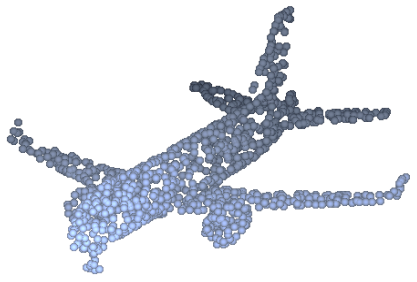
\includegraphics[scale=0.8]{point-cloud-aeroplane.png}}} \qquad
\vcenter{\hbox{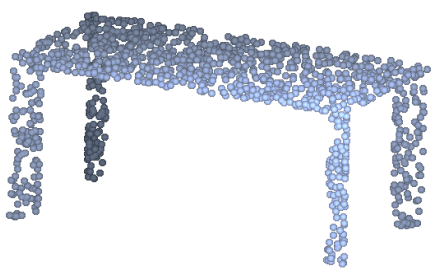
\includegraphics[scale=0.8]{point-cloud-desk.png}}}
\end{equation}
In a point cloud, it does not matter the order in which the points are presented, as inputs to the classifier function.  Such a function needs to be permutation invariant to a huge number of points.  More generally, see also these recent articles on the use of geometry and symmetry in deep learning: \cite{Bronstein2021} \cite{Bronstein2021a}.

From \cite{Zaheer2017a}: the \textbf{Kolmogorov–Arnold representation theorem} states that every multivariate continuous function can be represented as a sum of continuous functions of one variable:
\begin{equation}
f(x_1,... ,x_n) = \sum_{q=0}^{2n}\Phi_{q} \left(\sum_{p=1}^n \phi_{q,p}(x_p) \right)
\end{equation}
Their paper specialized the theorem to the case that every symmetric multivariate function can be represented as a sum of (the same) functions of one variable:
\begin{equation}
\label{symmetric-functions}
f(x_1, ..., x_n) = g(h(x_1) + ... + h(x_n))
\end{equation}
This leads to the following implementation using neural networks:
\begin{equation}
\vcenter{\hbox{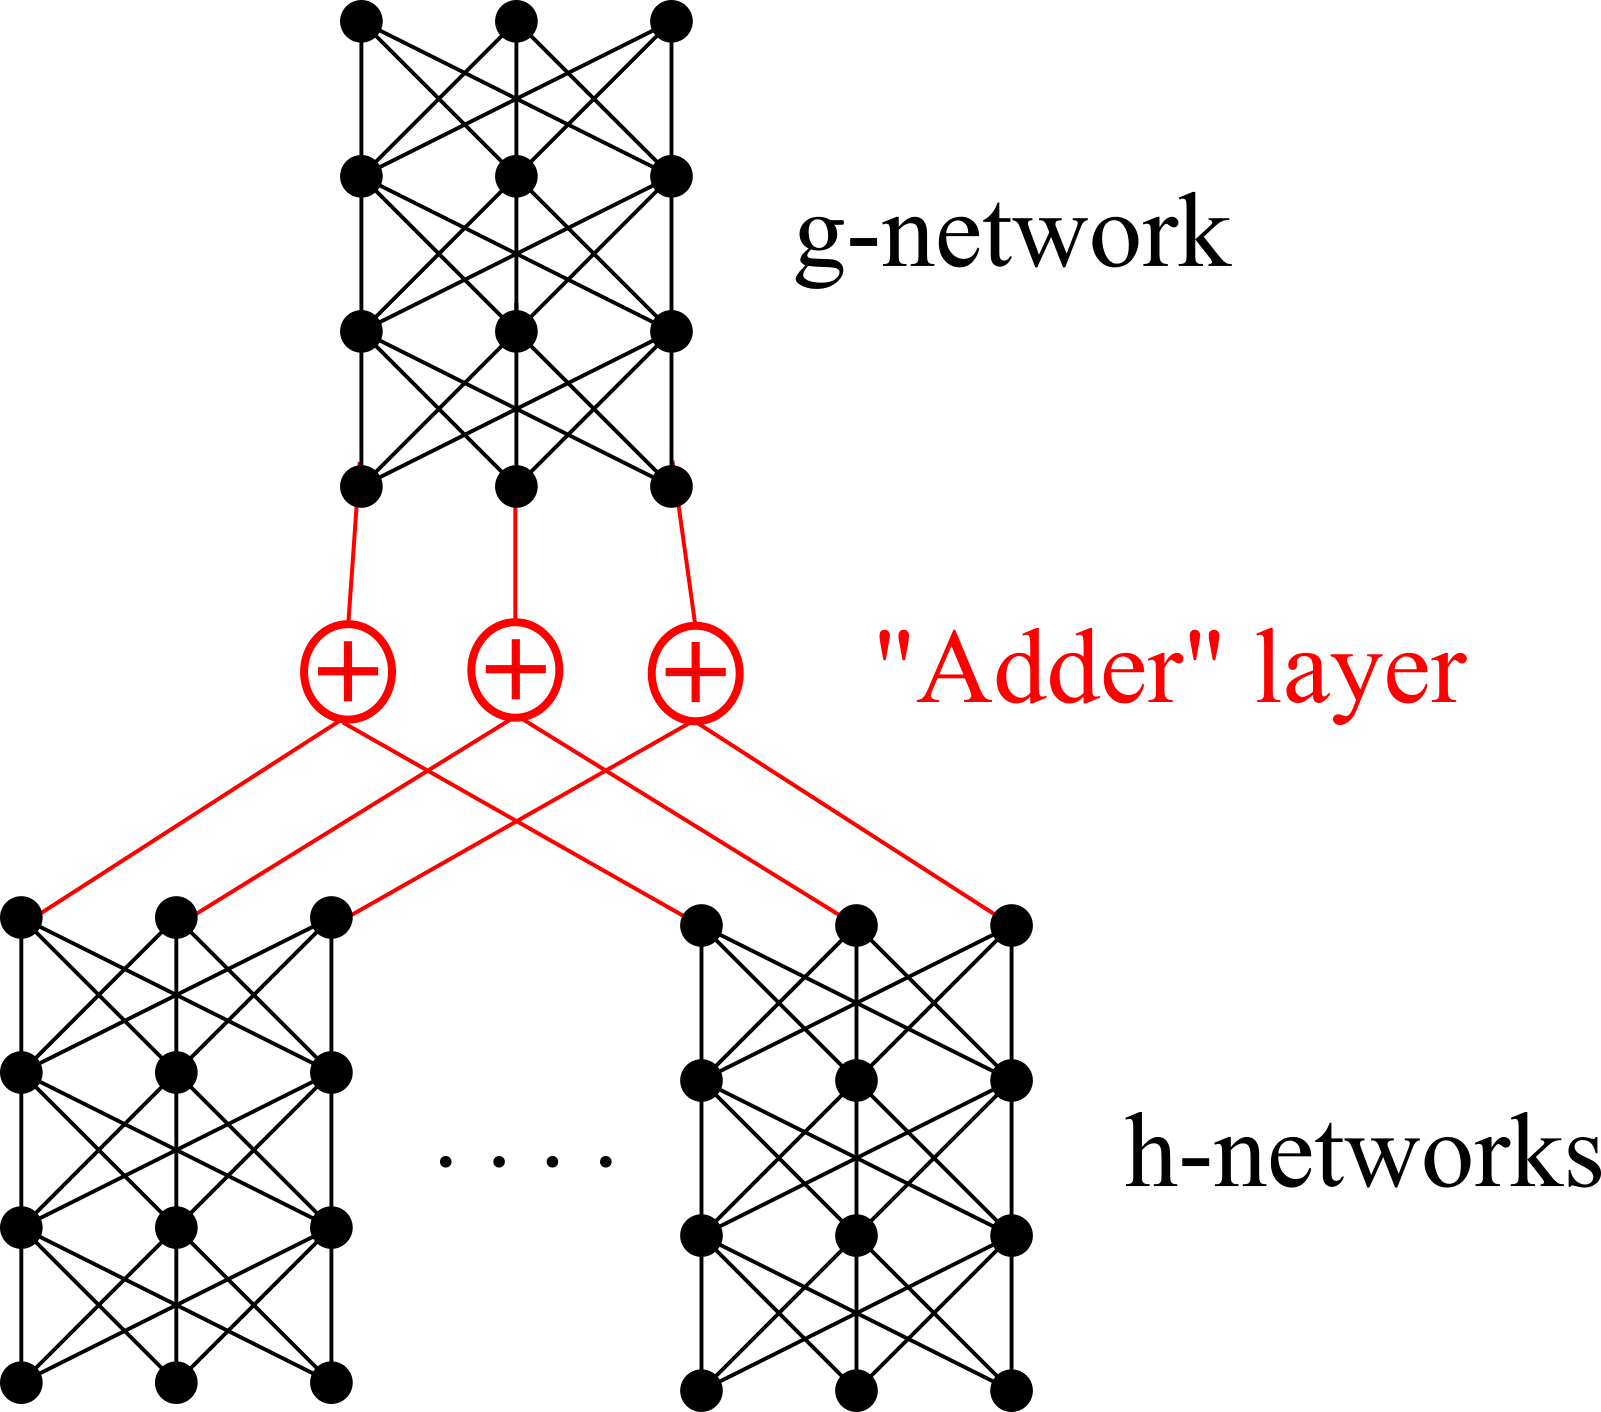
\includegraphics[scale=0.4]{g-and-h-networks.png}}}
\end{equation}
And this can be easily implemented with just a few lines of Tensorflow, see \S\ref{sec:experiment}.

\subsection{Why BERT is a Logic}

BERT (and its variants) are based on the Transformer architecture \cite{Devlin2018}, and Transformers are based solely on the Self-Attention mechanism \cite{Vaswani2017}.  In the following diagram \footnote{From blog article: Illustrated: Self-Attention
-- Step-by-step guide to self-attention with illustrations and code \\ https://towardsdatascience.com/illustrated-self-attention-2d627e33b20a }, one can verify that the Transformer is permutation-invariant (or more precisely, \textbf{equivariant}).  That is to say, for example, if input \#1 and \#2 are swapped, then output \#1 and \#2 would also be swapped:
\begin{equation}
\vcenter{\hbox{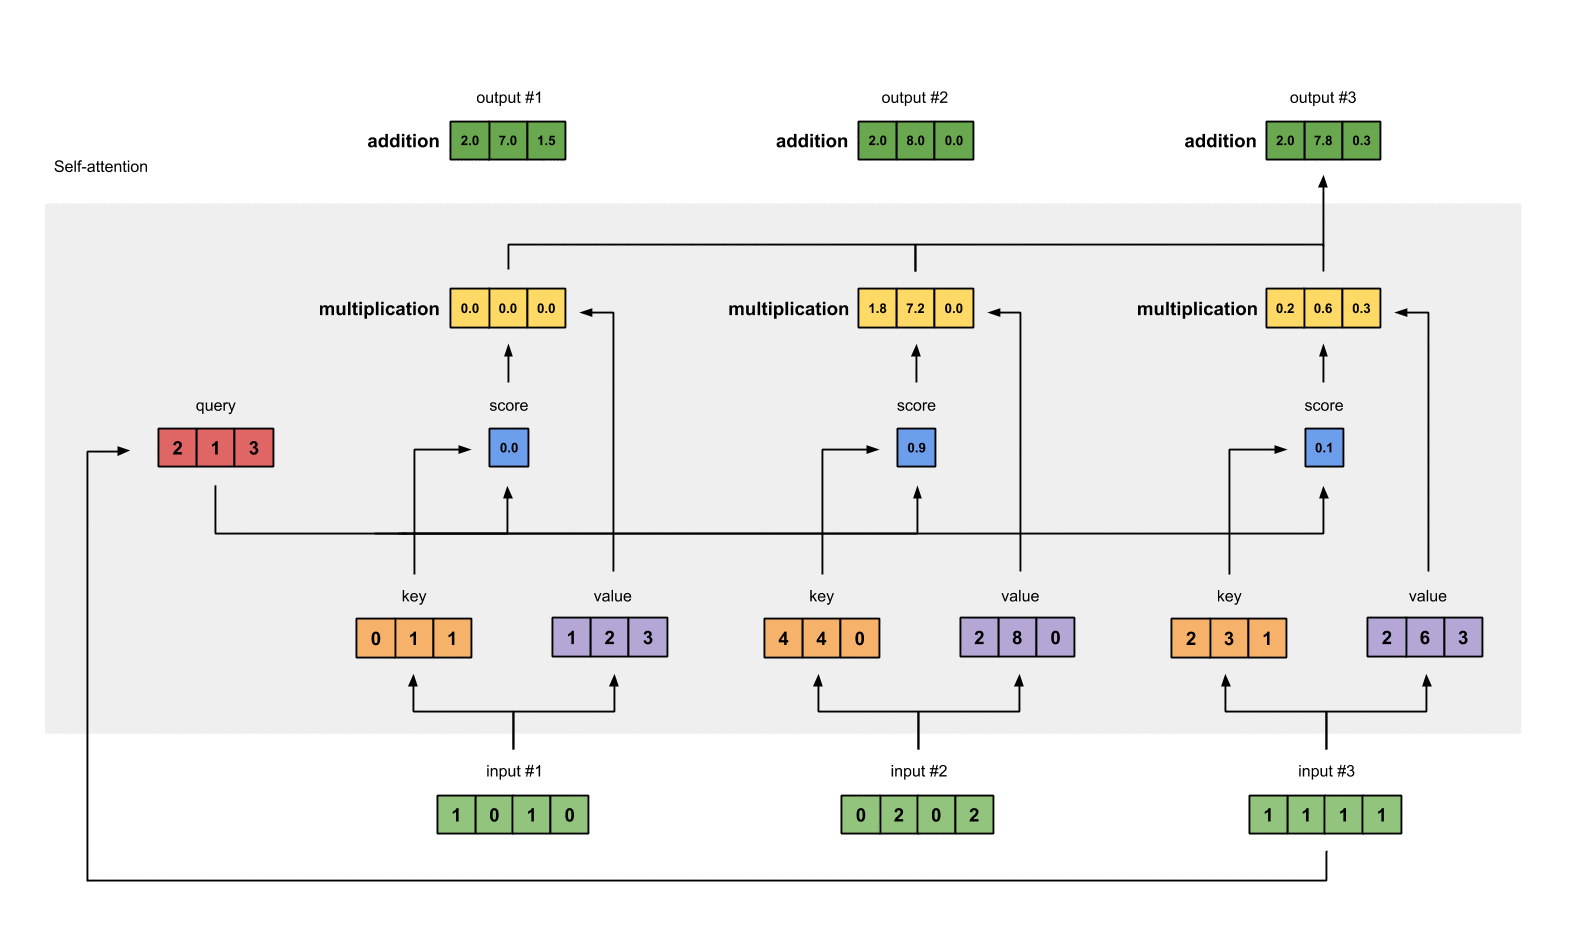
\includegraphics[scale=0.25]{self-attention.png}}}
\end{equation}
In other words, each Transformer layer takes $N$ inputs and produces $N$ equivariant outputs.  That is the same as saying that \textit{each} output is permutation-invariant in all its inputs.  As we explained in the last section, permutation invariance is the symmetry that characterizes a logic as having \textit{individual} propositions.

Below is a simplified diagram of an Attention layer.  The output is a new proposition that depends on the input objects, and thus, functions as a \textbf{predicate}:
\begin{equation}
\vcenter{\hbox{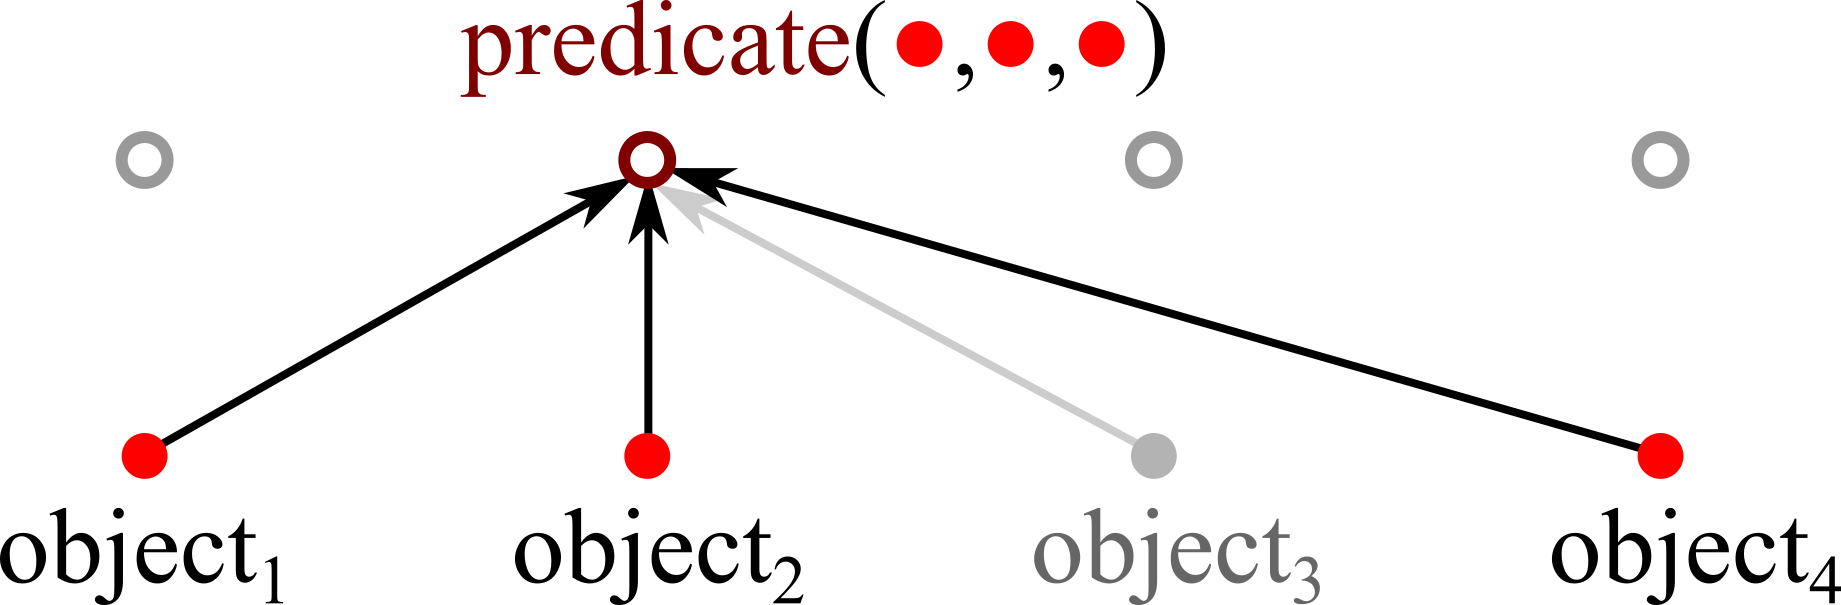
\includegraphics[scale=0.5]{attention-as-predicate.png}}}
\end{equation}

In \textbf{Multi-Head Attention}, the intermediate computations are duplicated multiple (eg, $M = 8$) times, each with their own weight matrices.  From the logic point of view, this amounts to duplicating $M$ logic rules per output.  But since the next layer still expects $N$ inputs, the $M$ outputs are combined into one, before the next stage.  Thus, from the logic point of view this merely increased the parameters \textit{within} a single logic rule, and seems not significant to increase the power of the logic rule-base.  Indeed, experimental results seem to confirm that multi-head attention is not particularly gainful towards performance.

A comment is in order here, about the choice of the word ``head''.  In logic programming (eg Prolog), one calls the conclusion of a logic rule its ``head'', such as \texttt{P} in \texttt{P :- Q,R,S}.  Perhaps the creators of BERT might have logic rules in mind?

\section{``No Free Lunch'' Theory}

In machine learning, ``No Free Lunch'' \cite{Wolpert1997} \cite{Alpaydin2020} refers to the fact that accelerating the search for a solution by ignoring one part of the search space (known as ''inductive bias'' \cite{Alpaydin2020}) is just as good as ignoring another part, if the solutions are believed to be evenly distributed in those regions.  For example, the symmetry proposed here reduces the search space by a factor of $1/n!$ where $n$ is the number of propositions in working memory.

The following conceptual diagram of the algorithmic search space illustrates the possibility that there might exist some form of logic that is drastically different from the symbolic logic currently known to humans:
\begin{equation}
\vcenter{\hbox{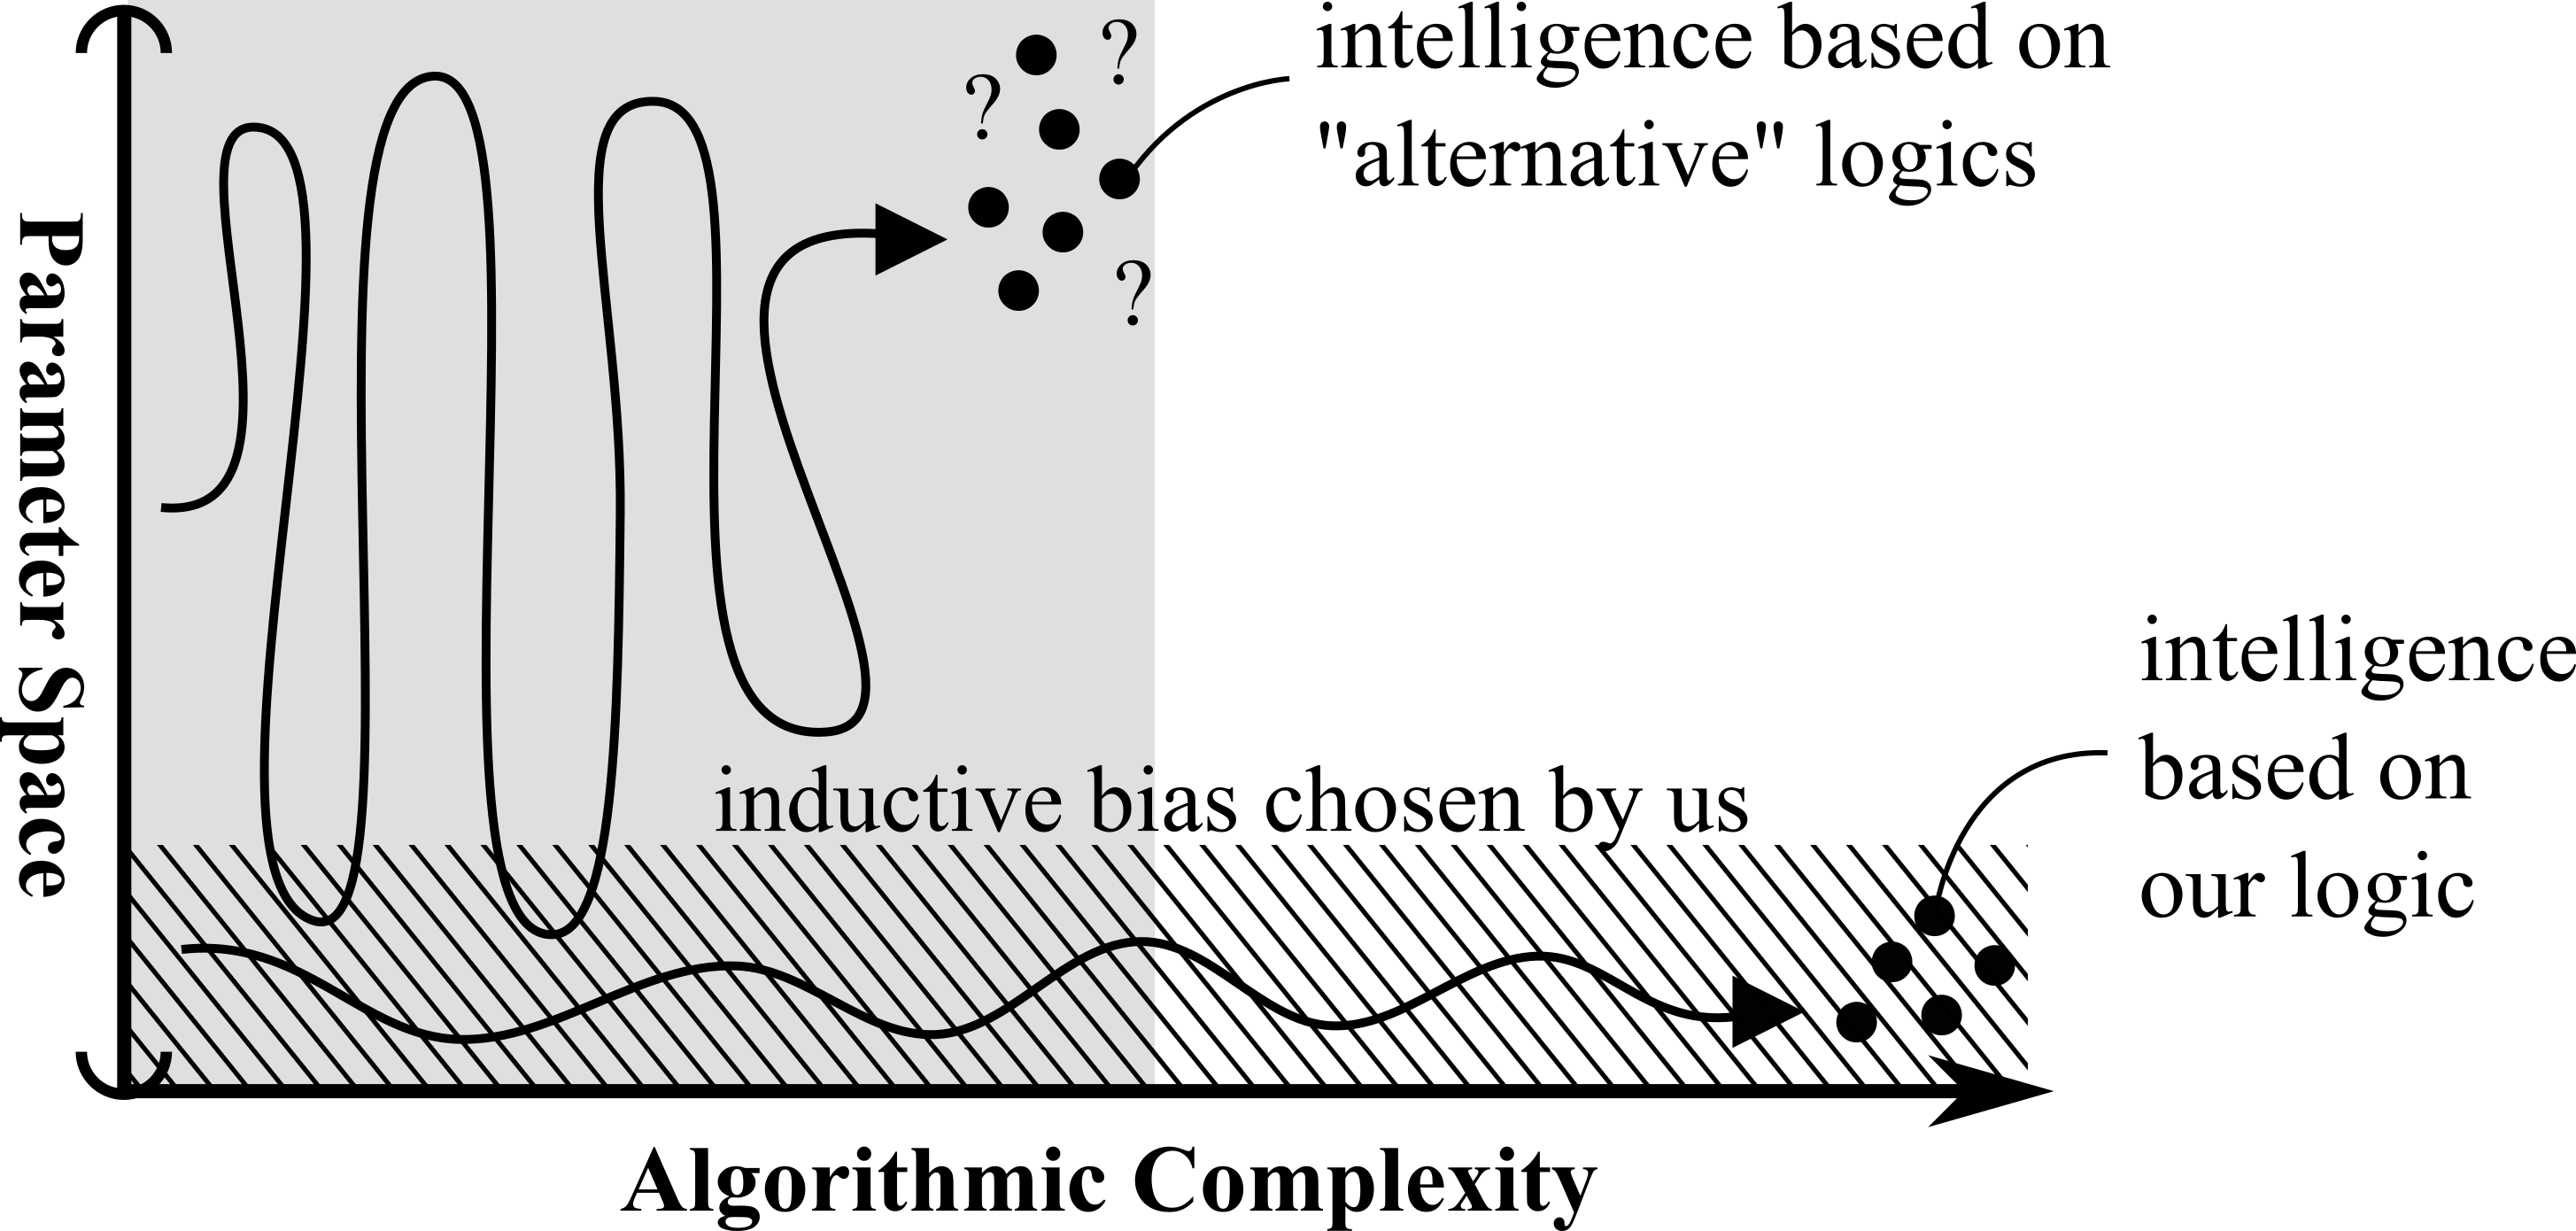
\includegraphics[scale=0.45]{no-free-lunch.png}}}
\end{equation}
but there is no efficient algorithm to find them (grey area is much larger than shaded area).  The permutation symmetry proposed in this paper forces our logic to be decomposable into \textbf{propositions}.  Such a logical form allows a mental state to be enumerated as a list of sentences (propositions), same as the ``linear'' structure of human \textbf{languages}.  If the AGI knowledge representation is linear (in the sequential sense) and symbolic, then it would not be far from our formulation -- all these logics belong to one big family.

But could there be drastically different logics?  One observes that pictures and music are not easily described by words, indeed they are 2-dimensional structures.  This suggests that the brain may use \textbf{multi-dimensional} arrays of features to represent the world.  Such a ``logic'' would be very different from sequential logic and it would be interesting and fruitful to analyze the relation between them.

\section{Experiment}
\label{sec:experiment}

A simple test \footnote{ Code with documentation is on GitHub: https://github.com/Cybernetic1/policy-gradient } of the symmetric neural network, under reinforcement learning (Policy Gradient \footnote{The Policy Gradient algorithm is chosen because it allows \textit{continuous} actions.  Other reinforcement learning algorithms require learning the value function over actions, and when the action space is not discrete such a value function cannot be represented by a table, but perhaps as a neural network.  However, it is not easy to find the \textit{maximum} of a neural network, which is required to choose the optimal action.  Policy Gradient avoids this because the policy function directly maps to actions.}), has been applied to the Tic-Tac-Toe game.

The state of the game is represented as a set of 9 propositions, where all propositions are initialized as ``null'' in the beginning.  During each step of the game, a new proposition is added to the set (ie. over-writing the null propositions).  Each proposition encodes who the player is, and which square $(i,j)$ she has chosen.  In other words, it is a predicate of the form: \texttt{move(player,i,j)}.  The neural network takes 9 propositions as input, and outputs a new proposition;  Thus it is a permutation-invariant function.

In comparison, the game state of traditional RL algorithms (eg. AlphaGo \cite{Silver2016} \cite{Silver2017} \cite{Pumperla2019}) usually is represented as a ``chessboard'' vector (eg. $3 \times 3$ in Tic-Tac-Toe, $8 \times 8$ in Chess, $19 \times 19 = 361$ in Go \footnote{In AlphaGo and AlphaZero, the algorithm makes use of several auxiliary ``feature planes'' that are also chessboard vectors, to indicate which stones have ``liberty'', ``ko'', etc.}).  This state vector is the same constant length even if there are very few pieces on the chessboard.  Our logic-based representation may offer some advantages over the board-vector representation, and likely induces a different ``way of reasoning'' about the game.

In our Tic-Tac-Toe experiment, convergence of learning is observed early on, but the algorithm fell short of achieving the highest score (19 instead of 20), and the score displayed unstable oscillating behavior after it got near the optimal value:
\begin{equation}
\vcenter{\hbox{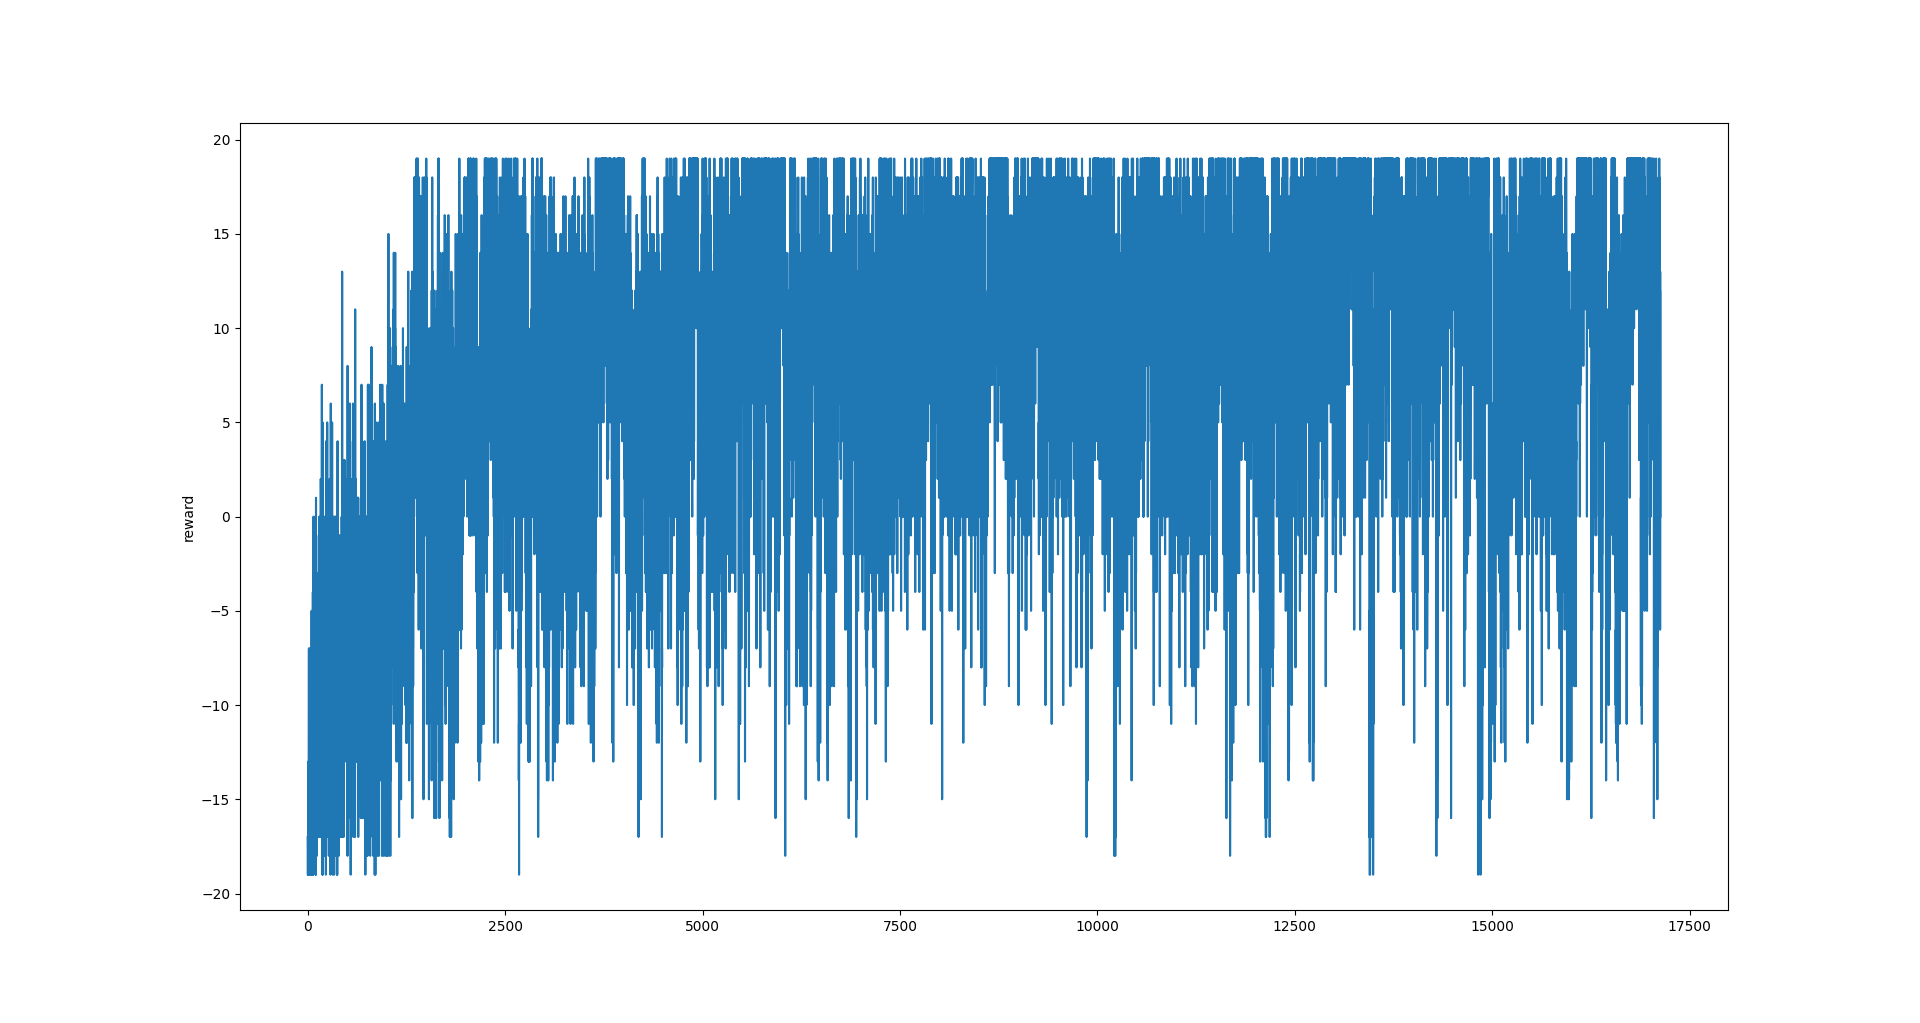
\includegraphics[scale=0.2]{TTT2-test4-convergence.png}}}
\end{equation}
In comparison, the board-vector version (also using policy gradient) fails to get near the highest score after 2 hours, and it also shows oscillatory behavior (suggesting the latter is due to the Policy Gradient algorithm).  Further investigation is needed, but this seems to be a promising start.

\section{Conclusion and Future Directions}

We described a minimal AGI with a logic that can derive one new proposition per iteration.  This seems sufficient to solve simple logic problems such as Tic-Tac-Toe.  As a next step, we would consider inference rules with multi-proposition conclusions.  The latter seems essential to \textbf{abductive} reasoning.  For example, one can deduce the concept ``apple'' from an array of visual features;  Conversely, the idea of an ``apple'' could also evoke in the mind a multitude of features, such as color, texture, taste, and the facts such as that it is edible, is a fruit, and that Alan Turing died from eating a poisoned apple (a form of episodic memory recall), and so on.  This many-to-many inference bears some similarity to the brain's computational mechanisms \cite{Rolls2016} \cite{Rolls2021} \cite{Boraud2020}.  The author is embarking on an abstract unifying AGI theory that makes references to (but not necessarily copying) brain mechanisms.

\section*{Acknowledgements}

Thanks Ben Goertzel for suggesting that neural networks are advantageous over pure symbolic logic because they have fast learning algorithms (by gradient descent).  That was at a time when ``deep learning'' was not yet a popular word.  Thanks Dmitri Tkatch for pointing me to existing research of symmetric neural networks.  Thanks Dr. 肖达 (Da Xiao) for explaining to me details of BERT. 

Also thanks to the following people for invaluable discussions over many years:  Ben Goertzel, Pei Wang (王培), Abram Demski, Russell Wallace, Juan Carlos Kuri Pinto, SeH, Jonathan Yan, and others.  Also thanks to all the university professors and researchers in Hong Kong (especially in the math departments, and their guests), strangers who taught me things on Zhihu.com (知乎), Quora.com, and StackOverflow.

\printbibliography

{\color{red}(To the editor:  Diagrams in this paper can be re-organized in the traditional format, please contact the author if this is desired.)}

\end{document}
